\documentclass{article}

\usepackage{graphicx}
\usepackage{listings}
\usepackage{color}

\definecolor{mygreen}{rgb}{0,0.6,0} 
\definecolor{mygray}{rgb}{0.5,0.5,0.5} 
\definecolor{mymauve}{rgb}{0.58,0,0.82}

%Scala
\lstdefinelanguage{scala}{
  morekeywords={abstract,case,catch,class,def,%
    do,else,extends,false,final,finally,%
    for,if,implicit,import,match,mixin,%
    new,null,object,override,package,%
    private,protected,requires,return,sealed,%
    super,this,throw,trait,true,try,%
    type,val,var,while,yield},
  otherkeywords={=>,<-,<\%,<:,>:,\#,@},
  sensitive=true,
  morecomment=[l]{//},
  morecomment=[n]{/*}{*/},
  morestring=[b]",
  morestring=[b]',
  morestring=[b]"""
}

% Default settings for code listings
\lstset{frame=tb,
  language=scala,
  aboveskip=3mm,
  belowskip=3mm,
  showstringspaces=false,
  columns=flexible,
  basicstyle={\small\ttfamily},
  numbers=none,
  numberstyle=\tiny\color{mygray},
  keywordstyle=\color{blue},
  commentstyle=\color{mygreen},
  stringstyle=\color{mymauve},
  frame=single,
  breaklines=true,
  breakatwhitespace=true
  tabsize=3
}

\title{Research Study - Metrics for code 'functional-ness' in Scala }
\date{\today}
\author{Alexandru Matei}

\begin{document}


\pagenumbering{gobble}
\maketitle

\newpage
\tableofcontents
\newpage

\pagenumbering{arabic}
\section{Introduction}
Functional programming started to get more traction in the last years, thanks to the growing adoption of Scala and Haskell in the software industry; we can see that Google trends shows a rising interest in functional programming languages (see figure \ref{fig:google-rank}). \par

\begin{figure}[h!]
  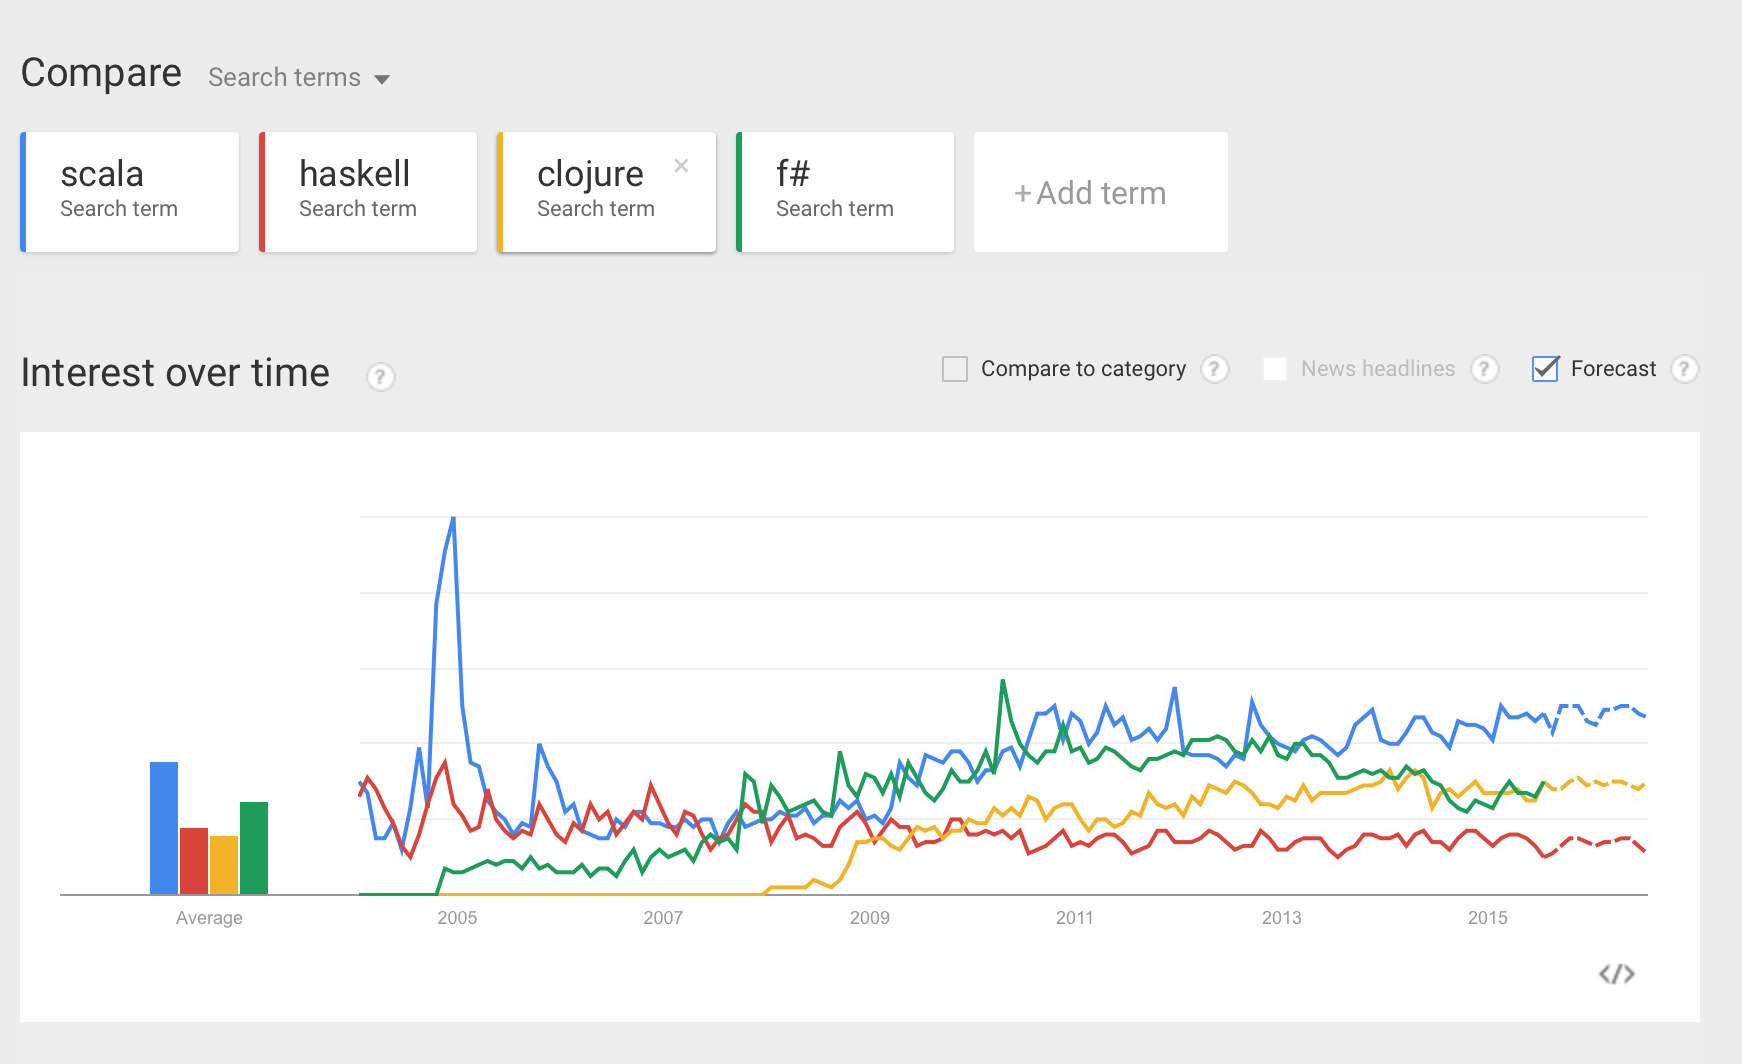
\includegraphics[width=\linewidth]{google-trends.png}
  \caption{Google search hits for programming languages - 2004 to July, 2015 }
  \label{fig:google-rank}
\end{figure}

Scala is one of the leading functional programming languages, over the last couple of years being adopted by large companies such as  Twitter(2009), Linkedin(2010), The Guardian, Foursquare. If we look at 'RedMonk Programming Languages Rankings'\cite{redmonk:1}, which is based on StackOverflow and Github analysis,  Scala occupies a worthy 14th position, being the first FP language in top . \par

\begin{figure}[h!]
  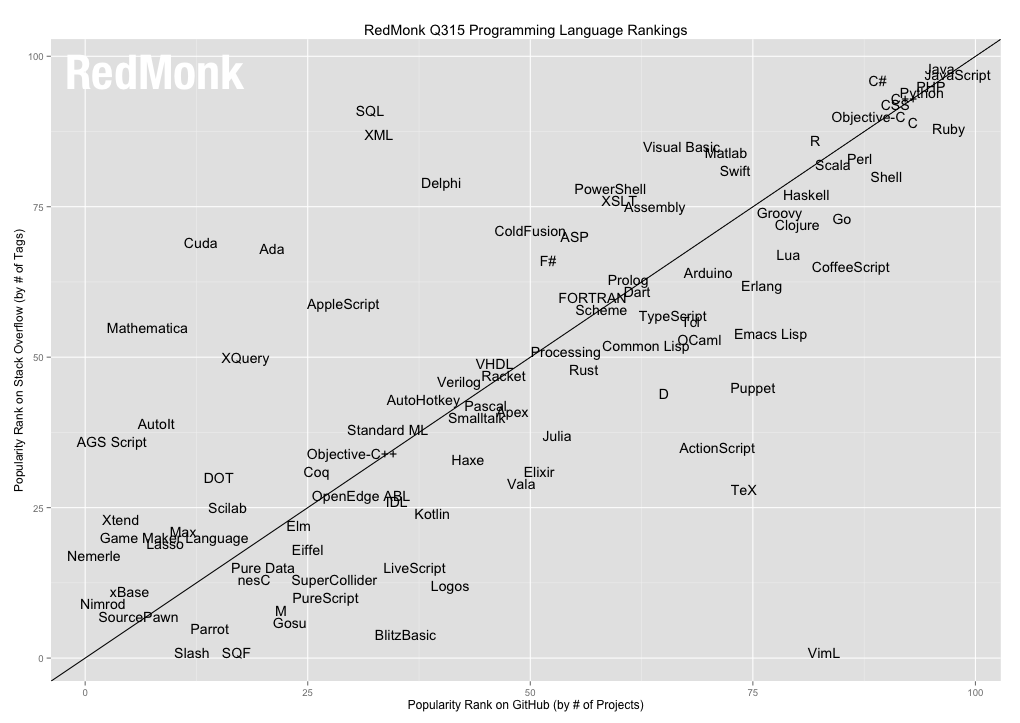
\includegraphics[width=\linewidth]{redmonk-rank.png}
  \caption{Redmonk rank of programming languages - June, 2015}
  \label{fig:redmonk-rank}
\end{figure}


One of its success factors is  Scala's JVM compatibility and code interoperability with Java, and the benefits that come along from  Java's well-estabilished eco-system. Another one might be that MOOCs  like Functional Programming in Scala \cite{scalastat:1} held  by the creator of Scala, Martin Odersky and Reactive Programming are one of the most popular online courses; the feedback from developers is really encouraging(see figure \ref{fig:interest}). \par

\begin{figure}[h!]
  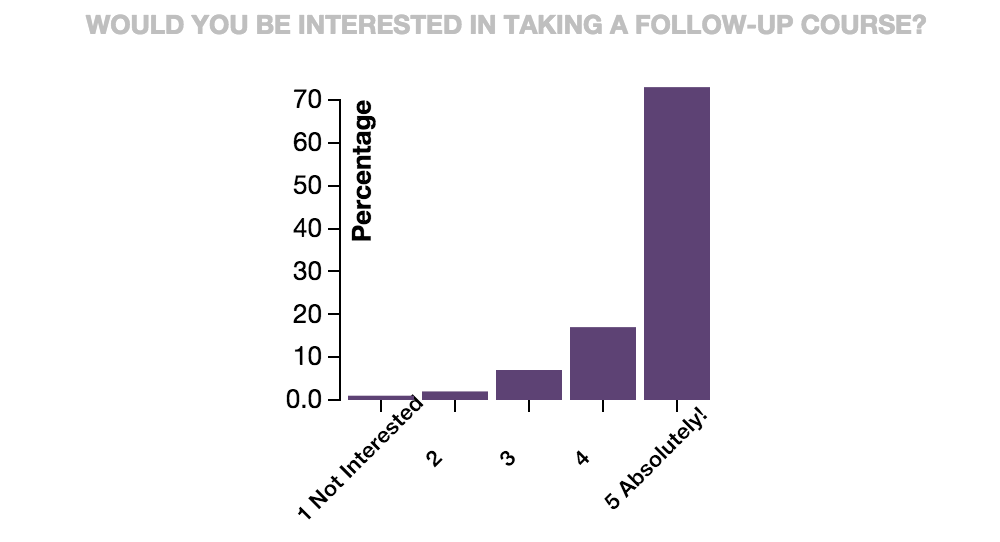
\includegraphics[width=\linewidth]{interest.png}
  \caption{Feedback FP in Scala course - interest in future courses on Scala (FP)}
  \label{fig:interest}
\end{figure}

Another reason why FP comes in handy nowadays is that multiprocessor architectures become ubiquitous and developers need to get more familiar with distributed and multi-threaded computing; programming with shared state has proven to be pretty difficult to reason about and functional programming offers to save a lot of headaches by removing shared state from the equation and providing better concurrency abstractions (Futures, Actors) and we should also consider  the exceptional distribution capabilities of map-reduce that FP offers. Although the programming paradigm was born more than 80 years ago, FP seems like a totally new way of thinking about software to modern day developers, having lots of secret gems left to be discovered. \par

\section {Problem description}
Scala is a hybrid programming lanaguage being both a functional language and an object oriented one ( cite http://www.scala-lang.org/what-is-scala.html). Using the features of functional programming should lead to less code which in turn usually leads to less bugs and better understandability. K. van den Berg Phd. thesis concludes that 'The results of the experiments show that the programs in a functional lan- guage took significantly less time to develop and were considerably more con- cise and easier to understand than the corresponding programs written in an imperative language' \cite{DBLP:journals/infsof/BergB95}. \par

Writing Scala code does not imply you are writing functional code;  there is no mechanism in the language that enforces a functional style of programming; so one can say he writes code in Scala so he uses FP when in fact his code base is entirely procedural. I was also put in such a position,  being one of the many  developers that  switched from an Object Oriented language(Java /C\#/C++xs etc.)  to a functional language such as Scala. So how can one figure out if his Scala code follows the FP principles or not? The classic approach is to ask a functional programming expert for code review, if you are lucky enough to have access to such valuable resources. Wouldn't it be nicer (and cheaper) to have a free tool that does the code review job for you? \par

The solution we propose is an automatic tool checker that would be able to asses one's code `functional-ness'; it should be able to guide the Scala programmer through the coding process and help him understand what features of FP he is using or missing on. We can imagine having a DSL for choosing which are the targeted FP properties for the analysis and receiving an detailed report on the analysis with further guidelines. \par

But what  qualifies a code as being functional? What are the specifics of a functional code? These are some of the questions that we have to answer first, in order to come up with metrics for code functional-ness.\par


\section {Methodology}
First of all we need to establish the characteristics of FP languages, taking Scala as an example. Only then we can elaborate further on the metrics and decide which ones are to be considered for the study. \par

We get to ask ourselves the following questions: `how much does a method uses functional programming concepts?` Does it contain only immutable data, so no shared state? Does it use higher order functions for data processing? Does a method use advanced features such as monadic comprehension? Does a method use functional-like constructs such as anonymous inner classes? \par

\subsection {Immutability}
If a variable/object is immutable then it's value never changes. That is a really usefull guarantee if one plans on going concurrent: any such value can be safely shared amongst treads since the value is read-only. Another advantage is the reduced aliasing between different parts of the program; one can say that immutable objects are easier to reason about and also their API is straight forward because you don't need to reason about internal state changes - everything is transparent compared to mutable objects that introduce opaqueness in reasoning about their possible states at different moments of time . \par
Scala encourages immutability through case classes, which provide a syntatic sugar for creating immutable objects (data structures). Case classes are regular classes which export their constructor parameters and which provide a recursive decomposition mechanism via pattern matching.

\begin{lstlisting} 
abstract class Pet
case class Dog(name:String) extends Pet 
case class Cat(name:String) extends Pet
case class Hippo(name:String, weight:Int) extends Pet

//Decomposition
def printPetType(pet:Pet): String= pet match{
  case Dog => "it's a Dog"
  case Cat => "it's a Cat"
  case Hippo => "it's a Hippo"
}
\end{lstlisting}

By default, case classes ar immutable but one can change some of fields to be mutable, although it is not recommended.\par

Declaring a variable as a 'val' prevents it for being reassigned; still, this doesn't guarantee that the object it is reffering to is immutable. Best transparency is obtained with using both val's and immutable objects: this is the recommended approach also when dealing with concurrency. Scala provides both mutable and immutable collections that can be found in packages scala.collection.mutable and scala.collection.immmutable repectively. By default, Scala always picks immutable collections. 

\begin{lstlisting} 
val x = 4
x = 5 //Reasignment to val generates error
\end{lstlisting}


So, in order to create an immutable Scala object, it is necessary to have all the fields declared as vals + all the values to be immutable objects in turn. Case classes make it more easier to accomplish that in as few lines of code as possible.

\subsection {Referential tranparency, pure functions}
An expression is referentially transparent (RT) if it can be replaced by its resulting value without changing the behavior of the program. This must be true regardless of where the expression is used in the program. Programming without side effects leads to referential transparency. An example:

\begin{lstlisting}
def f(x:Int)= x* 3
val z = f(3)
\\Now, whenever we use z in the code, we can safely
\\ replace it with f(3) without changing the result of the program
\end{lstlisting}

Pure functions evaluates to the same result given the same argument value(s) and they don't have any side effects. A better definition can be found in 'Functional Programming in Scala' by Chiusano and Bjarnason : 'A function f is pure if expression f(x) is referentially transparent for all referentially trasparent values x'.\par
Examples of pure functions in Scala include:
\begin{itemize}

 \item Methods on immutable collections such as map, drop, filter, take
 \item Methods like split, length on the String class
 \item Mathematical functions such as add, multiply \ldots
\end{itemize}
As a rule of thumb in Scala if a function has its return type Unit, then most probably it has side effects. 


\subsection {High-order functions}
One of the features pointed out by John Hughes \cite{DBLP:journals/cj/Hughes89} in 'Why Functional Programming Matters' are higher- order functions and lazy evaluation; Hughes argues that these two concepts greatly increase the modularity of software by providing novative ways (compared to other structured programming techniques) of 'gluing' modules together so programs can become more concise and easier to reason about. One other design pattern that was first approached in Haskel and targets modularity by emphasizing on composition is represented by monads which model the concept of a category (see \ref{monads}). \par 
Before we begin talking about high-order functions we should first understand what does an order of a function mean:

\begin{itemize}
\item Order 0: Non function data
\item Order 1: Functions with domain and range of order 0
\item Order 2: Functions with domain and range of order 1
\item Order k: Functions with domain and range of order k-1
\end{itemize}

So order 0 is represented by numbers, lists, characters, etc. Order 1 are functions wich work with order 0 data. So order 1 data are the well known functions that every programming language supports. 
Functions with an order grater than 1 are callled higher-order functions and they fall at least in on of the following categories:

\begin{itemize}
\item they take other functions as parameters
\item they return a function as a result
\end{itemize}

An example is the following apply function written in Scala, which takes a function (defined on integers that returns a string) and an integer as parameters and returns the function application over the integer value: \par

\begin{lstlisting} 
def apply(f: Int => String, v: Int) = f(v)
\end{lstlisting} 


Classical higher-order functions over lists :

\begin{itemize}
\item Mapping: Application of a function on all elements in a list
\item Filtering : Collection of elements from a list which satisfy a particular condition
\item Accumulation: Pair wise combination of the elements of a list to a value of
another type
\item Zipping: Combination of two lists to a single list
\end{itemize}
[http://people.cs.aau.dk/~normark/prog3-03/pdf/higher-order-fu.pdf]


\subsection {Monads}  \label{monads}
In Category Theory, a Monad is a functor equipped with a pair of natural transformations satisfying the laws of associativity and identity. In Scala, monads are just a parametric type M[T] with two operations, flatMap (or bind) and unit which also preserves associativity and identity. \par

\begin{lstlisting}
trait M[T]{
  def flatMap[U](f:T=>M[U]): M[U]
}

def unit[T](x:T): M[T]
\end{lstlisting}

\subsection {Lazy evaluation}
Lazy evaluation or call-by-need is the opposite of eager evaluation(call-by-value) and it is an evaluation strategy which delays the evaluation of an expression until it is needed and only then computes the result and caches it for further evaluations. \par
One advantage is the memory saving due to postponing the evaluation but it comes with a performance cost: you get faster intialization but later (when evaluation occurs) you suffer a performance penality.\par

Scala supports laziness by introducing the lazy keyword and call by name parameters. By default it supports strict evaluation in contrast with Haskell which is lazy by default.

\begin{lstlisting}
lazy val product = 100 * 30 // not evaluated
println(product.toString) // evaluated 


object Test {
   def main(args: Array[String]) {
        delayed(time());
   }

   def time() = {
      println("Getting time in nano seconds")
      System.nanoTime
   }
   def delayed( t: => Long ) = {
      println("In delayed method")
      println("Param: " + t)
      t
   }
}

\end{lstlisting}

\section {Literature study}

Current research on functional programming static analysis include Klass van den Berg \cite{DBLP:journals/infsof/BergB95} which studies the use cases of control-flow graphs in Miranda, a pure functional language, same as Haskell; the main focus is on program coprehensibility and they conclude that structured function definitions appear to be easier to understand by novice programmers. \par

Chris Ryder an Simon Thompson propose a series of metrics for Haskell functional programming language in order to reason about functions that may have an increased risk for errors and might need more rigurous testing \cite{RyderT05:TFP_2005_Intellect}. \par

Regarding Scala programming language, Basavaraju Muddu studies metrics for assessing Scala modularity; the study focuses on referential tranparency, functional purity and high order functions, some of the aspects that we will also use in our metrics to determine code functional-ness \cite{DBLP:conf/icse/MudduABP13}. To some extent, modularization metrics are a subset of the functional-ness metrics. \par

As for the industry there are already a couple of static analysis tools written for Scala : 
\begin{itemize}
\item 'ScalaStyle' that is a scala style checker  (implemented rules can be found at http://www.scalastyle.org/rules-0.7.0.html)
\item  ScapeGoat plugin (https://github.com/sksamuel/scalac-scapegoat-plugin) - signals suspicious language usage in code
\item  Wart remover https://github.com/puffnfresh/wartremover - linting tool
\item  HairyFotr/linger https://github.com/HairyFotr/linter
\item  Scala Abide https://github.com/scala/scala-abide - linting tool
\end{itemize}

Most of the previous research on functional programming metrics has been targeting program complexity, readability and maintability. Besavaraju Muddo takes the study a step further and developes metrics for studying modularization of FP programs. Static analyzers developed for Scala are mainly linting tools, to support detection of code smells and possible errors. \par


\section{Further Research}



Scala provides an API to extend its compiler through Scala compiler plugins; how they work is that they insert custom functionality at different stages of the compilation; of course this could lead to errors, if used improperly. Unfortunately, there are only a limited amount of resources online (http://lampwww.epfl.ch/~magarcia/ScalaCompilerCornerReloaded/) that talk about how to create plugins. \par
We have to first decide upon the patterns that are most relevant and study about the compiler support for performing such analysis (Scala compiler plug-ins). 



\newpage


\bibliography{citation} 
\bibliographystyle{alpha}

\end{document}





